% Chemostat snapshots for the visual simulation-loop figure (Supp. Fig. S2).
% Drawn at the same native TikZ units as Figure~\ref{fig:two-task-chain}c; subfigure cells
% downscale via \SimLoopVisCell + \resizebox (uniform scale of geometry and line weights).
% Fixed population layout: cross-feed pair (PopA/PopB) upper row; generalist PopC lower
% center (dies); PopD Task-A-only (lower left, $M_2$ persists); PopE Task-A-only
% (lower right, $M_2$ outflows). Six $M_1$ units inflow: four consumed in Task~A;
% one unused bottom-left persists; one unused top-right outflows.
\makeatletter
% Measure half-width (square) or radius (circle) from the rendered node shape.
\def\mccmchainbound@measure#1#2{%
  \pgfpointanchor{#1}{east}\pgf@xa=\pgf@x
  \pgfpointanchor{#1}{center}\pgf@xc=\pgf@x
  \pgfmathsetmacro{#2}{(\pgf@xa-\pgf@xc)/1cm}%
}
% L-infinity boundary on an axis-aligned square: #2=(...) target coordinate expression.
\def\mccmchainbound@square@i#1#2#3{%
  \coordinate (mccm@bnd@vec) at ($ (#2) - (#1.center) $);%
  \pgf@process{\pgfpointanchor{mccm@bnd@vec}{center}}%
  \pgfmathsetmacro{\mccm@dx}{\pgf@x/1cm}%
  \pgfmathsetmacro{\mccm@dy}{\pgf@y/1cm}%
  \pgfmathparse{abs(\mccm@dx)>=abs(\mccm@dy) ? (\mccm@dx>=0 ? 1 : -1) : (\mccm@dy>=0 ? 2 : -2)}%
  \pgfmathtruncatemacro{\mccm@anchnum}{\pgfmathresult}%
  \ifnum\mccm@anchnum=1 \def\mccm@anch{east}\else
    \ifnum\mccm@anchnum=-1 \def\mccm@anch{west}\else
      \ifnum\mccm@anchnum=2 \def\mccm@anch{north}\else
        \def\mccm@anch{south}\fi\fi\fi
  \coordinate (#3) at (#1.\mccm@anch);%
}
\def\mccmchainbound@square#1#2#3#4{%
  \mccmchainbound@square@i{#1}{#2.center}{#4}%
}
\def\mccmchainbound@squaretoc#1#2#3#4{%
  \mccmchainbound@square@i{#1}{#2}{#4}%
}
\def\mccmchainbound@circle#1#2#3#4{%
  \mccmchainbound@measure{#1}{\mccm@r}%
  \coordinate (#4) at ($(#1.center)!{\mccm@r cm}!(#2.center)$);%
}
\def\mccmchainbound@circletoc#1#2#3#4{%
  \mccmchainbound@measure{#1}{\mccm@r}%
  \coordinate (#4) at ($(#1.center)!{\mccm@r cm}!(#2)$);%
}
\def\mccmchainboundpoint#1#2#3#4#5{%
  \def\mccmchainbound@shape{#4}%
  \ifx\mccmchainbound@shape circle
    \mccmchainbound@circle{#1}{#2}{#3}{#5}%
  \else
    \mccmchainbound@square{#1}{#2}{#3}{#5}%
  \fi
}
\def\mccmchainboundpointtoc#1#2#3#4#5{%
  \def\mccmchainbound@shape{#4}%
  \ifx\mccmchainbound@shape circle
    \mccmchainbound@circletoc{#1}{#2}{#3}{#5}%
  \else
    \mccmchainbound@squaretoc{#1}{#2}{#3}{#5}%
  \fi
}
\def\mccmchainmetabarrowscale{0.58}
\def\mccmchainminiarrowscale{0.055}  % ~10% of featured metabolism arrowheads
\def\mccmchainthickarrowscale{0.70}
\def\mccmchainmetabtip{-{Stealth[scale=\mccmchainmetabarrowscale]}}
\def\mccmchainarrowcolorstop{0.74}  % colored gradient ends here
\def\mccmchainarrowshaftstop{0.78}  % colored shaft ends; head zone follows
\def\mccmchainarrowshorten{0.9pt}
\def\mccmchainminiarrowcolorstop{0.74}
\def\mccmchainminiarrowshaftstop{0.78}
\def\mccmchainminiarrowshorten{0.15pt}
\def\mccmchainheadmaskextend{1.1pt}  % bg cap past shortened path end
\def\mccmchainpipesarrowshorten{2.6pt}
\def\mccmchaingradsteps{20}
\def\mccmchaingradlast{19}
\def\mccmchainsegoverlap{0.40}
\colorlet{mccmchainmetabbg}{white}
\colorlet{mccmchainminimetabbg}{white}
\def\mccmchainmetabmaskwidth{1.24pt}
\def\mccmchainminimetabmaskwidth{0.42pt}
% Background under the head-only zone (colorstop -> sink).
\def\mccmchaindrawmetab@masktip#1#2{%
  \coordinate (mbMaskStart) at ($(#1)!\mccmchainarrowcolorstop!(#2)$);%
  \draw[line width=\mccmchainmetabmaskwidth, line cap=butt, draw=mccmchainmetabbg]
    (mbMaskStart) -- (#2);%
}
\def\mccmchaindrawminimetab@masktip#1#2{%
  \coordinate (mbMiniMaskStart) at ($(#1)!\mccmchainminiarrowcolorstop!(#2)$);%
  \draw[line width=\mccmchainminimetabmaskwidth, line cap=butt, draw=mccmchainminimetabbg]
    (mbMiniMaskStart) -- (#2);%
}
% Solid shaft bridge from gradient end to shaft stop (butt cap, no arrow).
\def\mccmchaindrawmetab@shaftbridge#1#2#3{%
  \coordinate (mbMetColorEnd) at ($(#1)!\mccmchainarrowcolorstop!(#2)$);%
  \coordinate (mbMetShaftEnd) at ($(#1)!\mccmchainarrowshaftstop!(#2)$);%
  \draw[mccmchainmetabline@butt, draw=#3] (mbMetColorEnd) -- (mbMetShaftEnd);%
}
\def\mccmchaindrawminimetab@shaftbridge#1#2#3{%
  \coordinate (mbMiniColorEnd) at ($(#1)!\mccmchainminiarrowcolorstop!(#2)$);%
  \coordinate (mbMiniShaftEnd) at ($(#1)!\mccmchainminiarrowshaftstop!(#2)$);%
  \draw[mccmchainminimetabline, line cap=butt, draw=#3]
    (mbMiniColorEnd) -- (mbMiniShaftEnd);%
}
% Tipped segment on head zone only, then hide any forward stub past Stealth.
\def\mccmchaindrawmetab@maskforward#1#2{%
  \draw[line width=\mccmchainmetabmaskwidth, line cap=butt, draw=mccmchainmetabbg]
    ($(#2)!-\mccmchainheadmaskextend!(#1)$) -- (#2);%
}
\def\mccmchaindrawminimetab@maskforward#1#2{%
  \draw[line width=\mccmchainminimetabmaskwidth, line cap=butt, draw=mccmchainminimetabbg]
    ($(#2)!-\mccmchainheadmaskextend!(#1)$) -- (#2);%
}
\def\mccmchaindrawmetab@head#1#2#3{%
  \draw[mccmchainmetabline@butt,
    -{Stealth[scale=\mccmchainmetabarrowscale, fill={#3}]},
    shorten >=\mccmchainarrowshorten, draw=#3] (#1) -- (#2);%
  \mccmchaindrawmetab@maskforward{#1}{#2}%
}
\def\mccmchaindrawminimetab@head#1#2#3{%
  \draw[mccmchainminimetabline, line cap=butt,
    -{Stealth[scale=\mccmchainminiarrowscale, fill={#3}]},
    shorten >=\mccmchainminiarrowshorten, draw=#3] (#1) -- (#2);%
  \mccmchaindrawminimetab@maskforward{#1}{#2}%
}
% Mask + head-only tip (#1=leg start for mask, #2=shaft end, #3=sink, #4=color).
\def\mccmchaindrawmetab@splithead#1#2#3#4{%
  \mccmchaindrawmetab@masktip{#1}{#3}%
  \mccmchaindrawmetab@head{#2}{#3}{#4}%
}
\def\mccmchaindrawminimetab@splithead#1#2#3#4{%
  \mccmchaindrawminimetab@masktip{#1}{#3}%
  \mccmchaindrawminimetab@head{#2}{#3}{#4}%
}
% Solid final leg: shaft body, bridge, then head only.
\def\mccmchaindrawmetab@finalleg#1#2#3{%
  \coordinate (mbMetShaftEnd) at ($(#1)!\mccmchainarrowshaftstop!(#2)$);%
  \draw[mccmchainmetabline@butt, draw=#3] (#1) -- (mbMetShaftEnd);%
  \mccmchaindrawmetab@splithead{#1}{mbMetShaftEnd}{#2}{#3}%
}
\def\mccmchaindrawminimetab@finalleg#1#2#3{%
  \coordinate (mbMiniShaftEnd) at ($(#1)!\mccmchainminiarrowshaftstop!(#2)$);%
  \draw[mccmchainminimetabline, line cap=butt, draw=#3] (#1) -- (mbMiniShaftEnd);%
  \mccmchaindrawminimetab@splithead{#1}{mbMiniShaftEnd}{#2}{#3}%
}
% Round cap fill at path corners / chunk joints (#2 = color).
\def\mccmchainmetab@joint#1#2{%
  \fill[#2] (#1) circle [radius=0.60pt];%
}
\def\mccmchainminimetab@joint#1#2{%
  \fill[#2] (#1) circle [radius=0.19pt];%
}
% Redraw a metabolite square above metabolism arrows at its port.
\def\mccmchainrestackmet#1#2{\node[#2] at (#1) {};}
\tikzset{
  mccmchainmetabline/.style={line width=1.12pt, line cap=round, line join=round},
  mccmchainmetabline@butt/.style={mccmchainmetabline, line cap=butt},
  mccmchainminimetabline/.style={line width=0.35pt, line cap=round, line join=round},
}
% #1=segment index, #2=1 on final chunk (body stops at bodystop)
\def\mccmchainmetab@segloc#1#2#3{%
  \ifnum#2=1
    \pgfmathsetmacro{\mccmchainlocA}{max(0, (#1-\mccmchainsegoverlap)*\mccmchainarrowcolorstop/\mccmchaingradsteps)}%
    \pgfmathsetmacro{\mccmchainlocB}{min(\mccmchainarrowcolorstop, (#1+1)*\mccmchainarrowcolorstop/\mccmchaingradsteps)}%
  \else
    \pgfmathsetmacro{\mccmchainlocA}{max(0, (#1-\mccmchainsegoverlap)/\mccmchaingradsteps)}%
    \pgfmathsetmacro{\mccmchainlocB}{min(1, (#1+1)/\mccmchaingradsteps)}%
  \fi
}
% Draw one gradient chunk; #1--#2 endpoints, #3=path offset in [0,1), #4=1 on final chunk
\def\mccmchaindrawmetab@chunk#1#2#3#4{%
  \ifnum#4=1
    \foreach \j in {0,1,...,\mccmchaingradlast} {%
      \mccmchainmetab@segloc{\j}{1}{}%
      \pgfmathsetmacro{\mccmchainuA}{#3+\mccmchainlocA/4}%
      \pgfmathsetmacro{\mccmchainuB}{#3+\mccmchainlocB/4}%
      \coordinate (mbMetPtA) at ($(#1)!{\mccmchainlocA}!(#2)$);%
      \coordinate (mbMetPtB) at ($(#1)!{\mccmchainlocB}!(#2)$);%
      \pgfmathsetmacro{\mccmchainmixval}{int(round(100*(1-0.5*(\mccmchainuA+\mccmchainuB))))}%
      \edef\mccmchainmixexp{\mccmchainmixval}%
      \ifnum\j=\mccmchaingradlast
        \def\mccmchaincapline{mccmchainmetabline@butt}%
      \else
        \def\mccmchaincapline{mccmchainmetabline}%
      \fi
      \draw[\mccmchaincapline,
        draw=mccmchaincA!\mccmchainmixexp!mccmchaincB] (mbMetPtA) -- (mbMetPtB);%
    }%
    \coordinate (mbMetShaftEnd) at ($(#1)!\mccmchainarrowshaftstop!(#2)$);%
    \mccmchaindrawmetab@shaftbridge{#1}{#2}{mccmchaincB}%
    \mccmchaindrawmetab@splithead{#1}{mbMetShaftEnd}{#2}{mccmchaincB};%
  \else
    \foreach \j in {0,1,...,\mccmchaingradlast} {%
      \mccmchainmetab@segloc{\j}{0}{}%
      \pgfmathsetmacro{\mccmchainuA}{#3+\mccmchainlocA/4}%
      \pgfmathsetmacro{\mccmchainuB}{#3+\mccmchainlocB/4}%
      \coordinate (mbMetPtA) at ($(#1)!{\mccmchainlocA}!(#2)$);%
      \coordinate (mbMetPtB) at ($(#1)!{\mccmchainlocB}!(#2)$);%
      \pgfmathsetmacro{\mccmchainmixval}{int(round(100*(1-0.5*(\mccmchainuA+\mccmchainuB))))}%
      \edef\mccmchainmixexp{\mccmchainmixval}%
      \draw[mccmchainmetabline,
        draw=mccmchaincA!\mccmchainmixexp!mccmchaincB] (mbMetPtA) -- (mbMetPtB);%
    }%
  \fi
}
% Metabolism path: boundary points toward the next node (works at any angle).
\def\mccmchaindrawmetabarrow@i#1#2#3#4#5#6#7#8{%
  \colorlet{mccmchaincA}{#5}%
  \colorlet{mccmchaincB}{#6}%
  \mccmchainboundpoint{#2}{#3}{0}{square}{mbMetSrc}%
  \mccmchainboundpoint{#3}{#2}{0}{circle}{mbMetOrgIn}%
  \coordinate (mbMetOrgCtr) at (#3.center);%
  \mccmchainboundpoint{#3}{#4}{0}{circle}{mbMetOrgOut}%
  \mccmchainboundpoint{#4}{#3}{0}{square}{mbMetSnk}%
  % Source->organism leg: single draw (calc foreach fails to render on this span).
  \draw[mccmchainmetabline, shorten <=0.6pt,
    draw=mccmchaincA] (mbMetSrc) -- (mbMetOrgIn);%
  \mccmchaindrawmetab@chunk{mbMetOrgIn}{mbMetOrgCtr}{0.25}{0}%
  \mccmchaindrawmetab@chunk{mbMetOrgCtr}{mbMetOrgOut}{0.5}{0}%
  \mccmchaindrawmetab@chunk{mbMetOrgOut}{mbMetSnk}{0.75}{1}%
  \mccmchainmetab@joint{mbMetOrgIn}{mccmchaincA!88!mccmchaincB}%
  \mccmchainmetab@joint{mbMetOrgCtr}{mccmchaincA!50!mccmchaincB}%
  \mccmchainmetab@joint{mbMetOrgOut}{mccmchaincA!12!mccmchaincB}%
}
\def\mccmchaindrawmetabarrow#1#2#3#4#5#6{%
  \mccmchaindrawmetabarrow@i{#1}{#2}{#3}{#4}{#5}{#6}{\mccmchainmballradius}{\mccmchainmballradius}%
}
% Like metabarrow but continues center -> sink (no radial exit onto the org rim).
\def\mccmchaindrawmetabarrowCtrSink#1#2#3#4#5#6{%
  \colorlet{mccmchaincA}{#5}%
  \colorlet{mccmchaincB}{#6}%
  \mccmchainboundpoint{#2}{#3}{0}{square}{mbMetSrc}%
  \mccmchainboundpoint{#3}{#2}{0}{circle}{mbMetOrgIn}%
  \coordinate (mbMetOrgCtr) at (#3.center);%
  \mccmchainboundpoint{#4}{#3}{0}{square}{mbMetSnk}%
  \draw[mccmchainmetabline, shorten <=0.6pt,
    draw=mccmchaincA] (mbMetSrc) -- (mbMetOrgIn);%
  \mccmchaindrawmetab@chunk{mbMetOrgIn}{mbMetOrgCtr}{0.25}{0}%
  \mccmchaindrawmetab@chunk{mbMetOrgCtr}{mbMetSnk}{0.5}{1}%
  \mccmchainmetab@joint{mbMetOrgIn}{mccmchaincA!88!mccmchaincB}%
  \mccmchainmetab@joint{mbMetOrgCtr}{mccmchaincA!50!mccmchaincB}%
}
\def\mccmchaindrawmetabarrowExt#1#2#3#4#5#6#7#8{%
  \mccmchaindrawmetabarrow@i{#1}{#2}{#3}{#4}{#5}{#6}{#7}{#8}%
}
% On-circle lane anchors: #1=org node, #2/#3=in/out coord names, #4=radius (cm), #5=height fraction.
\def\mccmchainorglanecoords#1#2#3#4#5{%
  \pgfmathsetmacro{\mccm@lanef}{#5}%
  \pgfmathsetmacro{\mccm@laney}{\mccm@lanef* (#4)}%
  \pgfmathsetmacro{\mccm@lanex}{sqrt(1-\mccm@lanef*\mccm@lanef)*(#4)}%
  \coordinate (#2) at ($(#1.center)+({-\mccm@lanex cm},{\mccm@laney cm})$);%
  \coordinate (#3) at ($(#1.center)+({\mccm@lanex cm},{\mccm@laney cm})$);%
}
% Dual-task lane: route through org above/below center (closer to midline than metabolite rows).
\def\mccmchainorglanefrac{0.48}  % |lane height| as fraction of org radius
\def\mccmchaindrawmetabarrowLane#1#2#3#4#5#6#7{%
  \colorlet{mccmchaincA}{#5}%
  \colorlet{mccmchaincB}{#6}%
  \makeatletter
  \pgfpointanchor{#3}{center}\pgf@ya=\pgf@y
  \pgfpointanchor{#2}{center}\pgf@yb=\pgf@y
  \pgfmathsetmacro{\mccm@dy}{(\pgf@yb-\pgf@ya)/1cm}%
  \makeatother
  \pgfmathsetmacro{\mccm@lanef}{\mccmchainorglanefrac}%
  \ifdim\mccm@dy pt<0pt
    \pgfmathsetmacro{\mccm@lanef}{-\mccm@lanef}%
  \fi
  \mccmchainbound@measure{#3}{\mccm@orgr}%
  \pgfmathsetmacro{\mccm@lanex}{sqrt(1-\mccm@lanef*\mccm@lanef)*\mccm@orgr}%
  \pgfmathsetmacro{\mccm@laney}{\mccm@lanef*\mccm@orgr}%
  \coordinate (#1@In) at ($(#3.center)+({-\mccm@lanex cm},{\mccm@laney cm})$);%
  \coordinate (#1@Out) at ($(#3.center)+({\mccm@lanex cm},{\mccm@laney cm})$);%
  \coordinate (#1@Mid) at ($(#3.center)+(0 cm,{\mccm@laney cm})$);%
  \mccmchainboundpointtoc{#2}{#1@In}{0}{square}{#1@Src}%
  \mccmchainboundpoint{#4}{#3}{0}{square}{#1@Snk}%
  \draw[mccmchainmetabline, shorten <=0.6pt, draw=mccmchaincA]
    (#1@Src) -- (#1@In);%
  \mccmchaindrawmetab@chunk{#1@In}{#1@Mid}{0.25}{0}%
  \mccmchaindrawmetab@chunk{#1@Mid}{#1@Out}{0.5}{0}%
  \mccmchaindrawmetab@chunk{#1@Out}{#1@Snk}{0.75}{1}%
  \mccmchainmetab@joint{#1@In}{mccmchaincA!88!mccmchaincB}%
  \mccmchainmetab@joint{#1@Mid}{mccmchaincA!50!mccmchaincB}%
  \mccmchainmetab@joint{#1@Out}{mccmchaincA!12!mccmchaincB}%
}


\def\ChemostatSnapNativeXMin{-0.88}
\def\ChemostatSnapNativeXMax{9.98}
\def\ChemostatSnapNativeYMin{-0.48}
\def\ChemostatSnapNativeYMax{2.92}

\def\ChemostatSnapRefTankLW{0.9pt}
\def\ChemostatSnapRefMetabLW{1.12pt}
\def\ChemostatSnapRefDeathLW{0.85pt}
\def\ChemostatSnapRefCrossfeedLW{0.85pt}
\def\ChemostatSnapRefPipeShorten{2.6pt}
\def\ChemostatSnapRefMetabShorten{0.6pt}
\def\ChemostatSnapRefInflowMoneOffset{0.21}

% S2 glyph sizes vs.\ Fig.~\ref{fig:two-task-chain}c reference: organisms +30\%, metabolites $-$30\%.
\def\ChemostatSnapMballSize{3.85pt}
\def\ChemostatSnapMballSharedSize{4.9pt}
\def\ChemostatSnapOrgSize{10.4pt}
\def\ChemostatSnapOrgMutSize{9.1pt}
\def\ChemostatSnapOrgSmallSize{8.45pt}
\def\ChemostatSnapOrgEnergySize{15.6pt}
\def\ChemostatSnapOrgDupMutSize{8.45pt}

% Energy panel (S4 step 5) is scaled narrower than chemostat cells so row heights match.
\def\SimLoopVisEnergyWidthScale{0.56}

% Fixed population layout: PopA/PopB cross-feed (upper); PopC generalist (lower, dies);
% PopD Task-A-only (lower left, $M_2$ persists); PopE Task-A-only (lower right, $M_2$ outflows).
\def\ChemostatSnapPopAx{3.15}
\def\ChemostatSnapPopAy{2.08}
\def\ChemostatSnapPopBx{6.05}
\def\ChemostatSnapPopBy{2.08}
\def\ChemostatSnapPopCx{4.60}
\def\ChemostatSnapPopCy{0.52}
% PopD Task-A-only producer (lower left); pool $M_2$ remains after outflow.
\def\ChemostatSnapPopDx{2.45}
\def\ChemostatSnapPopDy{0.62}
% PopE Task-A-only producer (lower right); pool $M_2$ leaves via outflow.
\def\ChemostatSnapPopEx{7.15}
\def\ChemostatSnapPopEy{0.55}

% Persistent $M_2$ pool from PopD (remains after outflow / end of generation).
\def\ChemostatSnapUnusedMtwoX{2.18}
\def\ChemostatSnapUnusedMtwoY{1.02}
% Outflowing $M_2$ pool from PopE (closer to exit; flushed at chemostat outflow).
\def\ChemostatSnapPersistMtwoEX{7.42}
\def\ChemostatSnapPersistMtwoEY{1.02}

% Shared environmental $M_2$ for the bottom generalist (between upper and lower rows).
\def\ChemostatSnapPoolMtwoX{4.60}
\def\ChemostatSnapPoolMtwoY{1.15}

% $M_1$ pool destinations after resource inflow (six units per generation).
\def\ChemostatSnapPoolMoneAX{2.43}
\def\ChemostatSnapPoolMoneAY{2.18}
\def\ChemostatSnapPoolMoneCX{3.68}
\def\ChemostatSnapPoolMoneCY{0.56}
\def\ChemostatSnapPoolMoneDX{1.77}
\def\ChemostatSnapPoolMoneDY{0.68}
\def\ChemostatSnapPoolMoneEX{6.42}
\def\ChemostatSnapPoolMoneEY{0.58}
% Persistent unused $M_1$ (bottom left; remains after outflow).
\def\ChemostatSnapPoolMoneUnusedX{1.10}
\def\ChemostatSnapPoolMoneUnusedY{0.30}
% Outflowing unused $M_1$ (top right; flushed at chemostat outflow).
\def\ChemostatSnapPoolMoneOutflowX{7.82}
\def\ChemostatSnapPoolMoneOutflowY{2.58}
\def\ChemostatSnapInflowMoneOutX{-0.78}
% Evenly spaced external intake stack (top to bottom; shared by init and inflow).
\def\ChemostatSnapInflowStackTop{2.62}
\def\ChemostatSnapInflowStackBot{0.22}
\def\ChemostatSnapTrunkFlowArrowScale{0.95}  % direction markers on horizontal intake/outflow trunks
% Initialize Run intake routing (independent of Resource Inflow).
\def\ChemostatSnapInitTrunkXa{-0.42}
\def\ChemostatSnapInitMergeXshift{0.24}
\def\ChemostatSnapInitMergeCpStack{0.30}
\def\ChemostatSnapInitMergeCpTrunk{0.20}
\def\ChemostatSnapInitBranchBend{0.38}
\def\ChemostatSnapInitTrunkEnd{7.15}    % PopE $x$ (rightmost init branch cap)

\newif\ifChemostatSnapInitTrunkXeSet
\ChemostatSnapInitTrunkXeSetfalse

\newcommand{\ChemostatSnapInitTrunkXeReset}{%
  \global\ChemostatSnapInitTrunkXeSetfalse
}

\newcommand{\ChemostatSnapInitTrunkXeNote}[1]{%
  \ifChemostatSnapInitTrunkXeSet
    \pgfmathsetmacro{\ChemostatSnapInitTrunkXe}{max(\ChemostatSnapInitTrunkXe,#1)}%
  \else
    \pgfmathsetmacro{\ChemostatSnapInitTrunkXe}{#1}%
    \global\ChemostatSnapInitTrunkXeSettrue
  \fi
}

\newcommand{\ChemostatSnapInitTrunkXeDraw}[2]{%
  \pgfmathsetmacro{\csinitmergex}{\ChemostatSnapInitTrunkXa+\ChemostatSnapInitMergeXshift}%
  \ifChemostatSnapInitTrunkXeSet
    \ChemostatSnapIntakeTrunkDraw{#1}{\csinitmergex}{\ChemostatSnapInitTrunkXe}{#2}%
  \fi
}

% Resource Inflow intake routing (independent of Initialize Run).
\def\ChemostatSnapInflowTrunkXa{-0.42}
\def\ChemostatSnapInflowMergeXshift{0.24}
\def\ChemostatSnapInflowMergeCpStack{0.30}
\def\ChemostatSnapInflowMergeCpTrunk{0.20}
\def\ChemostatSnapInflowBranchBend{0.38}
\def\ChemostatSnapInflowTrunkEnd{7.82}   % outflow-bound $M_1$ pool $x$ (rightmost inflow branch cap)

\newif\ifChemostatSnapInflowTrunkXeSet
\ChemostatSnapInflowTrunkXeSetfalse

\newcommand{\ChemostatSnapInflowTrunkXeReset}{%
  \global\ChemostatSnapInflowTrunkXeSetfalse
}

\newcommand{\ChemostatSnapInflowTrunkXeNote}[1]{%
  \ifChemostatSnapInflowTrunkXeSet
    \pgfmathsetmacro{\ChemostatSnapInflowTrunkXe}{max(\ChemostatSnapInflowTrunkXe,#1)}%
  \else
    \pgfmathsetmacro{\ChemostatSnapInflowTrunkXe}{#1}%
    \global\ChemostatSnapInflowTrunkXeSettrue
  \fi
}

\newcommand{\ChemostatSnapInflowTrunkXeDraw}[2]{%
  \pgfmathsetmacro{\csinflowmergex}{\ChemostatSnapInflowTrunkXa+\ChemostatSnapInflowMergeXshift}%
  \ifChemostatSnapInflowTrunkXeSet
    \ChemostatSnapIntakeTrunkDraw{#1}{\csinflowmergex}{\ChemostatSnapInflowTrunkXe}{#2}%
  \fi
}
% Outflow manifold (mirror of inflow: branches on the left, external stack on the right).
\def\ChemostatSnapOutflowTrunkXe{8.18}   % outlet-side reference $x$ (mirror of \ChemostatSnapInflowTrunkXa)
\def\ChemostatSnapOutflowMergeXshift{0.24}  % stack merges land this far left of trunk right end
\def\ChemostatSnapOutflowMergeStackPull{0.95}  % vertical tangent pull toward trunk (stack-side CP)
\def\ChemostatSnapOutflowMergeTrunkPull{0.78}  % horizontal tangent pull along trunk (trunk-side CP)
\def\ChemostatSnapOutflowStackX{9.62}    % external outflow stack column
\def\ChemostatSnapOutflowStackDy{0.42}   % vertical spacing between outflow-stack glyphs
\def\ChemostatSnapOutflowBranchBend{0.38}  % trunk-to-vertical corner radius (outflow branches)
\def\ChemostatSnapOutflowTrunkCap{8.18}  % branch tee cap ($x$; mirror of \ChemostatSnapInflowTrunkEnd)

\newif\ifChemostatSnapOutflowTrunkXwSet
\ChemostatSnapOutflowTrunkXwSetfalse

\newcommand{\ChemostatSnapOutflowTrunkXwReset}{%
  \global\ChemostatSnapOutflowTrunkXwSetfalse
}

\newcommand{\ChemostatSnapOutflowTrunkXwNote}[1]{%
  \ifChemostatSnapOutflowTrunkXwSet
    \pgfmathsetmacro{\ChemostatSnapOutflowTrunkXw}{min(\ChemostatSnapOutflowTrunkXw,#1)}%
  \else
    \pgfmathsetmacro{\ChemostatSnapOutflowTrunkXw}{#1}%
    \global\ChemostatSnapOutflowTrunkXwSettrue
  \fi
}

\newcommand{\ChemostatSnapOutflowTrunkXwNoteNode}[2]{%
  \makeatletter
  \pgfpointanchor{#1}{center}\pgf@ya=\pgf@y
  \pgfmathsetmacro{\csoutflownodecy}{\pgf@ya/1cm}%
  \makeatother
  \pgfmathsetmacro{\csoutflownodeabove}{int(\csoutflownodecy>\mccmchainpipey)}%
  \makeatletter
  \ifnum\csoutflownodeabove=1
    \pgfpointanchor{#1}{south}\pgf@xa=\pgf@x
  \else
    \pgfpointanchor{#1}{north}\pgf@xa=\pgf@x
  \fi
  \pgfmathsetmacro{\csoutflownodex}{\pgf@xa/1cm}%
  \makeatother
  \pgfmathsetmacro{\csoutflownodetee}{min(\csoutflownodex, #2)}%
  \ChemostatSnapOutflowTrunkXwNote{\csoutflownodetee}%
}

\newcommand{\ChemostatSnapOutflowTrunkDraw}{%
  \pgfmathsetmacro{\csoutflowmergex}{\ChemostatSnapOutflowTrunkXe-\ChemostatSnapOutflowMergeXshift}%
  \ifChemostatSnapOutflowTrunkXwSet
    % Left end at leftmost branch junction (teex+bend; noted in \ChemostatSnapOutflowBranch).
    \pgfmathsetmacro{\csoutflowtrunkxwdraw}{min(\csoutflowmergex,\ChemostatSnapOutflowTrunkXw)}%
    \draw[csoutflowline, gray!65!black, line cap=butt]
      (\csoutflowtrunkxwdraw,\mccmchainpipey)
      -- (\csoutflowmergex,\mccmchainpipey);%
    \ChemostatSnapTrunkFlowArrows{\csoutflowtrunkxwdraw}{\csoutflowmergex}{gray!65!black}%
  \fi
  \draw[cspipe, gray!65!black, shorten >=\ChemostatSnapRefPipeShorten]
    (\csoutflowmergex,\mccmchainpipey) -- (csOutlet);%
}

\newcommand{\ChemostatSnapInflowStackY}[2]{%
  \pgfmathsetmacro{\csinflowstacktop}{\ChemostatSnapInflowStackTop}%
  \pgfmathsetmacro{\csinflowstackbot}{\ChemostatSnapInflowStackBot}%
  \pgfmathsetmacro{\csinflowstackindex}{#1}%
  \pgfmathsetmacro{\csinflowstackcount}{#2}%
  \pgfmathsetmacro{\csinflowstackstep}{(\csinflowstacktop-\csinflowstackbot)/max(1,\csinflowstackcount-1)}%
  \pgfmathsetmacro{\csinflowstacky}{\csinflowstacktop-\csinflowstackindex*\csinflowstackstep}%
}

% Init panel only: center PopC (stack slot 2) on the intake valve; two organisms above and below.
\newcommand{\ChemostatSnapInitStackY}[1]{%
  \pgfmathsetmacro{\csinitstackindex}{#1}%
  \pgfmathsetmacro{\csinitstackstep}{0.60}%
  \pgfmathsetmacro{\csinitstackcenter}{2}%
  \pgfmathsetmacro{\csinflowstacky}{\mccmchainpipey + (\csinitstackcenter-\csinitstackindex)*\csinitstackstep}%
}

% $M_2$ shared between cross-feeding specialists PopA and PopB (upper row).
\def\ChemostatSnapCrossfeedMtwoX{4.60}
\def\ChemostatSnapCrossfeedMtwoY{2.18}

% Offspring below the cross-feed row (reused in later panels).
\def\ChemostatSnapDupAx{3.55}
\def\ChemostatSnapDupAy{1.20}
\def\ChemostatSnapDupBx{5.85}
\def\ChemostatSnapDupBy{0.88}

\newcommand{\ChemostatSnapStyles}{%
  \tikzset{
    csmball/.style={rectangle, minimum size=\ChemostatSnapMballSize, inner sep=0pt},
    csmballMone/.style={csmball, draw=blue!70!black, fill=blue!22},
    csmballMtwo/.style={csmball, draw=yellow!55!black, fill=yellow!35},
    csmballShared/.style={csmball, draw=yellow!55!black, fill=yellow!38,
      minimum size=\ChemostatSnapMballSharedSize},
    csmballWaste/.style={csmball, draw=gray!65!black, fill=gray!18},
    csorg/.style={circle, draw=teal!55!black, fill=teal!14,
      minimum size=\ChemostatSnapOrgSize, inner sep=0pt},
    csorgMut/.style={circle, draw=none, fill=magenta!38,
      minimum size=\ChemostatSnapOrgMutSize, inner sep=0pt,
      append after command={\pgfextra{\ChemostatSnapMutBorder{\tikzlastnode}}}},
    csorgSmall/.style={csorg, minimum size=\ChemostatSnapOrgSmallSize},
    cspipe/.style={
      ->, thick,
      >={Stealth[scale=0.70]}},
    csmetab/.style={
      ->,
      line width=\ChemostatSnapRefMetabLW,
      line cap=round, line join=round,
      >={Stealth[scale=0.58]}},
    csinflowline/.style={
      dashed,
      line width=\ChemostatSnapRefMetabLW,
      line cap=round,
      line join=round,
      blue!65!black},
    csorginflowline/.style={
      dashed,
      line width=\ChemostatSnapRefMetabLW,
      line cap=round,
      line join=round,
      teal!55!black},
    csoutflowline/.style={
      dashed,
      line width=\ChemostatSnapRefMetabLW,
      line cap=round,
      line join=round},
    csinflow/.style={
      csinflowline,
      ->,
      >={Stealth[scale=0.58]}},
    csorginflow/.style={
      csorginflowline,
      ->,
      >={Stealth[scale=0.58]}},
    csoutflow/.style={
      csoutflowline,
      ->,
      >={Stealth[scale=0.58]}},
    csorgsplit/.style={->, thin},
    cscrossfeedbox/.style={draw=gray!60, dotted,
      line width=\ChemostatSnapRefCrossfeedLW,
      rounded corners=4pt, inner sep=0.22cm, fill=none},
  }%
}

\def\ChemostatSnapMutBorder#1{%
  \draw
    let \p1=(#1.east), \p2=(#1.west),
        \n1={0.5*(\x1-\x2)},
        \n2={max(0.30pt, 0.35*\n1)}
    in [line width=\n2, draw=magenta!80!black, line cap=round]
      (#1.center) ++(58:\n1) arc (58:122:\n1)
      (#1.center) ++(-32:\n1) arc (-32:32:\n1)
      (#1.center) ++(238:\n1) arc (238:302:\n1)
      (#1.center) ++(148:\n1) arc (148:212:\n1);%
}

% Parent--offspring split arrow along the center-to-center line.
\newcommand{\ChemostatSnapOrgSplit@frac}[2]{%
  \pgfpointanchor{#1}{center}%
  \pgfmathsetmacro{\csax}{\pgf@x/1cm}\pgfmathsetmacro{\csay}{\pgf@y/1cm}%
  \pgfpointanchor{#2}{center}%
  \pgfmathsetmacro{\csbx}{\pgf@x/1cm}\pgfmathsetmacro{\csby}{\pgf@y/1cm}%
  \pgfpointanchor{#1}{east}%
  \pgfmathsetmacro{\csex}{\pgf@x/1cm}%
  \pgfmathsetmacro{\csOrgSplitR}{abs(\csex-\csax)}%
  \pgfmathsetmacro{\csOrgSplitDx}{\csbx-\csax}%
  \pgfmathsetmacro{\csOrgSplitDy}{\csby-\csay}%
  \pgfmathsetmacro{\csOrgSplitD}{max(0.001, sqrt(\csOrgSplitDx*\csOrgSplitDx+\csOrgSplitDy*\csOrgSplitDy))}%
  \pgfmathsetmacro{\csOrgSplitFrac}{\csOrgSplitR/\csOrgSplitD}%
}
\newcommand{\ChemostatSnapOrgSplit}[3]{%
  \begingroup
  \ChemostatSnapOrgSplit@frac{#1}{#2}%
  \edef\csOrgSplitFracFrom{\csOrgSplitFrac}%
  \ChemostatSnapOrgSplit@frac{#2}{#1}%
  \edef\csOrgSplitFracTo{\csOrgSplitFrac}%
  \draw[csorgsplit, #3]
    ($(#1.center)!\csOrgSplitFracFrom!(#2.center)$)
    --
    ($(#2.center)!\csOrgSplitFracTo!(#1.center)$);
  \endgroup
}

\newcommand{\ChemostatSnapRestackMone}[1]{\mccmchainrestackmet{#1}{csmballMone}}
\newcommand{\ChemostatSnapRestackMtwo}[1]{\mccmchainrestackmet{#1}{csmballMtwo}}
\newcommand{\ChemostatSnapRestackWaste}[1]{\mccmchainrestackmet{#1}{csmballWaste}}
\newcommand{\ChemostatSnapRestackShared}[1]{\mccmchainrestackmet{#1}{csmballShared}}
% Gradient metabolism arrow through organism center (steps 2--4).
\newcommand{\ChemostatSnapMetabThroughOrg}[6]{%
  \mccmchaindrawmetabarrow{#1}{#2}{#3}{#4}{#5}{#6}%
}
% Task~A when $M_2$ pool is not collinear with $M_1$ (center exits toward sink).
\newcommand{\ChemostatSnapMetabThroughOrgCtrSink}[6]{%
  \mccmchaindrawmetabarrowCtrSink{#1}{#2}{#3}{#4}{#5}{#6}%
}
% Curved lane above/below organism (step~5 energy panel; optional motifs).
\newcommand{\ChemostatSnapMetabLane}[6]{%
  \mccmchaindrawmetabarrowLane{#1}{#2}{#3}{#4}{#5}{#6}{u}%
}

\newcommand{\ChemostatSnapTank}{%
  \def\mccmchaintankbot{-0.48}%
  \def\mccmchaintanktop{2.85}%
  \def\mccmchainpipeh{0.105}%
  \def\mccmchainstub{0.28}%
  \def\mccmchainrimd{0.09}%
  \def\mccmchainrimflare{0.055}%
  \def\mccmchaintankr{0.14}%
  \pgfmathsetmacro{\mccmchainpipey}{0.5*(\mccmchaintankbot+\mccmchaintanktop)}%
  \pgfmathsetmacro{\mccmchainbarrelbot}{\mccmchainpipey-\mccmchainpipeh}%
  \pgfmathsetmacro{\mccmchainbarreltop}{\mccmchainpipey+\mccmchainpipeh}%
  \pgfmathsetmacro{\mccmchainrimbot}{\mccmchainbarrelbot-\mccmchainrimflare}%
  \pgfmathsetmacro{\mccmchainrimtop}{\mccmchainbarreltop+\mccmchainrimflare}%
  \pgfmathsetmacro{\mccmchainbarrelL}{0.75-\mccmchainstub}%
  \pgfmathsetmacro{\mccmchainrimL}{\mccmchainbarrelL-\mccmchainrimd}%
  \pgfmathsetmacro{\mccmchainbarrelR}{8.45+\mccmchainstub}%
  \pgfmathsetmacro{\mccmchainrimR}{8.45+\mccmchainstub+\mccmchainrimd}%
  \coordinate (csInlet) at (\mccmchainrimL,\mccmchainpipey);%
  \coordinate (csOutlet) at (\mccmchainrimR,\mccmchainpipey);%
  \path[fill=gray!5, draw=gray!55, line width=\ChemostatSnapRefTankLW]
    (\mccmchainrimL,\mccmchainrimbot) -- (\mccmchainrimL,\mccmchainrimtop)
    -- (\mccmchainbarrelL,\mccmchainrimtop) -- (\mccmchainbarrelL,\mccmchainbarreltop)
    -- (0.75,\mccmchainbarreltop)
    -- (0.75,{\mccmchaintanktop-\mccmchaintankr})
    arc (180:90:\mccmchaintankr)
    -- (8.45-\mccmchaintankr,\mccmchaintanktop)
    arc (90:0:\mccmchaintankr)
    -- (8.45,\mccmchainbarreltop)
    -- (\mccmchainbarrelR,\mccmchainbarreltop) -- (\mccmchainbarrelR,\mccmchainrimtop)
    -- (\mccmchainrimR,\mccmchainrimtop) -- (\mccmchainrimR,\mccmchainrimbot)
    -- (\mccmchainbarrelR,\mccmchainrimbot) -- (\mccmchainbarrelR,\mccmchainbarrelbot)
    -- (8.45,\mccmchainbarrelbot)
    -- (8.45,{\mccmchaintankbot+\mccmchaintankr})
    arc (0:-90:\mccmchaintankr)
    -- (0.75+\mccmchaintankr,\mccmchaintankbot)
    arc (-90:-180:\mccmchaintankr)
    -- (0.75,{\mccmchaintankbot+\mccmchaintankr})
    -- (0.75,\mccmchainbarrelbot)
    -- (\mccmchainbarrelL,\mccmchainbarrelbot) -- (\mccmchainbarrelL,\mccmchainrimbot)
    -- cycle;%
}

\newcommand{\ChemostatSnapPopFive}{%
  \node[csorg] (csPopA) at (\ChemostatSnapPopAx,\ChemostatSnapPopAy) {};%
  \node[csorg] (csPopB) at (\ChemostatSnapPopBx,\ChemostatSnapPopBy) {};%
  \node[csorg] (csPopC) at (\ChemostatSnapPopCx,\ChemostatSnapPopCy) {};%
  \node[csorg] (csPopD) at (\ChemostatSnapPopDx,\ChemostatSnapPopDy) {};%
  \node[csorg] (csPopE) at (\ChemostatSnapPopEx,\ChemostatSnapPopEy) {};%
}

\newcommand{\ChemostatSnapPopFour}{%
  \ChemostatSnapPopFive
}

\newcommand{\ChemostatSnapPopThree}{%
  \ChemostatSnapPopFive
}

\newcommand{\ChemostatSnapPopSurvivors}{%
  \node[csorg] (csPopA) at (\ChemostatSnapPopAx,\ChemostatSnapPopAy) {};%
  \node[csorg] (csPopB) at (\ChemostatSnapPopBx,\ChemostatSnapPopBy) {};%
  \node[csorg] (csPopD) at (\ChemostatSnapPopDx,\ChemostatSnapPopDy) {};%
  \node[csorg] (csPopE) at (\ChemostatSnapPopEx,\ChemostatSnapPopEy) {};%
}

\newcommand{\ChemostatSnapPopAfterDup}{%
  \node[csorg] (csPopA) at (\ChemostatSnapPopAx,\ChemostatSnapPopAy) {};%
  \node[csorgMut, minimum size=\ChemostatSnapOrgDupMutSize] (csDupA) at (\ChemostatSnapDupAx,\ChemostatSnapDupAy) {};%
  \node[csorg] (csPopB) at (\ChemostatSnapPopBx,\ChemostatSnapPopBy) {};%
  \node[csorg] (csDupB) at (\ChemostatSnapDupBx,\ChemostatSnapDupBy) {};%
  \node[csorg] (csPopD) at (\ChemostatSnapPopDx,\ChemostatSnapPopDy) {};%
  \node[csorg] (csPopE) at (\ChemostatSnapPopEx,\ChemostatSnapPopEy) {};%
}

\newcommand{\ChemostatSnapPopAfterDupOnly}{%
  \node[csorg] (csPopA) at (\ChemostatSnapPopAx,\ChemostatSnapPopAy) {};%
  \node[csorg, minimum size=\ChemostatSnapOrgDupMutSize] (csDupA) at (\ChemostatSnapDupAx,\ChemostatSnapDupAy) {};%
  \node[csorg] (csPopB) at (\ChemostatSnapPopBx,\ChemostatSnapPopBy) {};%
  \node[csorg, minimum size=\ChemostatSnapOrgDupMutSize] (csDupB) at (\ChemostatSnapDupBx,\ChemostatSnapDupBy) {};%
  \node[csorg] (csPopD) at (\ChemostatSnapPopDx,\ChemostatSnapPopDy) {};%
  \node[csorg] (csPopE) at (\ChemostatSnapPopEx,\ChemostatSnapPopEy) {};%
}

\newcommand{\ChemostatSnapPopAfterOutflow}{%
  \node[csorg] (csPopA) at (\ChemostatSnapPopAx,\ChemostatSnapPopAy) {};%
  \node[csorgMut, minimum size=\ChemostatSnapOrgDupMutSize] (csDupA) at (\ChemostatSnapDupAx,\ChemostatSnapDupAy) {};%
  \node[csorg] (csPopB) at (\ChemostatSnapPopBx,\ChemostatSnapPopBy) {};%
  \node[csorg] (csPopD) at (\ChemostatSnapPopDx,\ChemostatSnapPopDy) {};%
  \node[csorg] (csPopE) at (\ChemostatSnapPopEx,\ChemostatSnapPopEy) {};%
}

\newcommand{\ChemostatSnapTrunkFlowArrows}[3]{%
  \foreach \t in {0.28, 0.58, 0.86} {%
    \pgfmathsetmacro{\csarrowx}{#1 + \t * (#2 - #1)}%
    \pgfmathsetmacro{\csarrowtip}{\csarrowx+0.20}%
    \ifdim\csarrowtip pt>\dimexpr#2 pt\relax
      \pgfmathsetmacro{\csarrowlen}{max(0.04, #2 - \csarrowx)}%
      \draw[-{Stealth[scale=\ChemostatSnapTrunkFlowArrowScale]}, #3, line width=\ChemostatSnapRefMetabLW]
        (\csarrowx,\mccmchainpipey) -- ++(\csarrowlen,0);%
    \else
      \draw[-{Stealth[scale=\ChemostatSnapTrunkFlowArrowScale]}, #3, line width=\ChemostatSnapRefMetabLW]
        (\csarrowx,\mccmchainpipey) -- ++(0.20,0);%
    \fi
  }%
}

\newcommand{\ChemostatSnapIntakeTrunkDraw}[4]{%
  \draw[#1, line cap=butt]
    (#2,\mccmchainpipey)
    -- (#3,\mccmchainpipey);%
  \ChemostatSnapTrunkFlowArrows{#2}{#3}{#4}%
}

\newcommand{\ChemostatSnapInitMerge}[3]{%
  \pgfmathsetmacro{\csinitmergex}{\ChemostatSnapInitTrunkXa+\ChemostatSnapInitMergeXshift}%
  \pgfmathsetmacro{\csinitmergecxone}{\ChemostatSnapInflowMoneOutX+\ChemostatSnapInitMergeCpStack}%
  \pgfmathsetmacro{\csinitmergecxtwo}{\csinitmergex-\ChemostatSnapInitMergeCpTrunk}%
  \draw[#1, shorten <=\ChemostatSnapRefMetabShorten]
    (#2.east)
    .. controls (\csinitmergecxone,#3) and (\csinitmergecxtwo,\mccmchainpipey) ..
    (\csinitmergex,\mccmchainpipey);%
}

\newcommand{\ChemostatSnapInitBranch}[5]{%
  \pgfmathsetmacro{\csinflowpooly}{#4}%
  \pgfmathsetmacro{\csinflowabove}{int(\csinflowpooly>\mccmchainpipey)}%
  \makeatletter
  \ifnum\csinflowabove=1
    \pgfpointanchor{#2}{south}\pgf@xa=\pgf@x \pgf@ya=\pgf@y
  \else
    \pgfpointanchor{#2}{north}\pgf@xa=\pgf@x \pgf@ya=\pgf@y
  \fi
  \pgfmathsetmacro{\csinflowedgex}{\pgf@xa/1cm}%
  \pgfmathsetmacro{\csinflowedgey}{\pgf@ya/1cm}%
  \makeatother
  \pgfmathsetmacro{\csinitmergex}{\ChemostatSnapInitTrunkXa+\ChemostatSnapInitMergeXshift}%
  \pgfmathsetmacro{\csinflowteex}{max(\csinitmergex, min(\csinflowedgex, #5))}%
  \pgfmathsetmacro{\csinitjunction}{\csinflowteex-\ChemostatSnapInitBranchBend}%
  \ChemostatSnapInitTrunkXeNote{\csinitjunction}%
  \ifnum\csinflowabove=1
    \draw[#1, shorten <=\ChemostatSnapRefMetabShorten]
      (#2.south)
      -- (\csinflowedgex,\csinflowedgey)
      -- (\csinflowedgex,\mccmchainpipey+\ChemostatSnapInitBranchBend)
      .. controls (\csinflowedgex,\mccmchainpipey)
                  and (\csinitjunction,\mccmchainpipey) ..
      (\csinitjunction,\mccmchainpipey);%
  \else
    \draw[#1, shorten <=\ChemostatSnapRefMetabShorten]
      (#2.north)
      -- (\csinflowedgex,\csinflowedgey)
      -- (\csinflowedgex,\mccmchainpipey-\ChemostatSnapInitBranchBend)
      .. controls (\csinflowedgex,\mccmchainpipey)
                  and (\csinitjunction,\mccmchainpipey) ..
      (\csinitjunction,\mccmchainpipey);%
  \fi
}

\newcommand{\ChemostatSnapInflowMerge}[3]{%
  \pgfmathsetmacro{\csinflowmergex}{\ChemostatSnapInflowTrunkXa+\ChemostatSnapInflowMergeXshift}%
  \pgfmathsetmacro{\csinflowmergecxone}{\ChemostatSnapInflowMoneOutX+\ChemostatSnapInflowMergeCpStack}%
  \pgfmathsetmacro{\csinflowmergecxtwo}{\csinflowmergex-\ChemostatSnapInflowMergeCpTrunk}%
  \draw[#1, shorten <=\ChemostatSnapRefMetabShorten]
    (#2.east)
    .. controls (\csinflowmergecxone,#3) and (\csinflowmergecxtwo,\mccmchainpipey) ..
    (\csinflowmergex,\mccmchainpipey);%
}

\newcommand{\ChemostatSnapInflowBranch}[5]{%
  \pgfmathsetmacro{\csinflowpooly}{#4}%
  \pgfmathsetmacro{\csinflowabove}{int(\csinflowpooly>\mccmchainpipey)}%
  \makeatletter
  \ifnum\csinflowabove=1
    \pgfpointanchor{#2}{south}\pgf@xa=\pgf@x \pgf@ya=\pgf@y
  \else
    \pgfpointanchor{#2}{north}\pgf@xa=\pgf@x \pgf@ya=\pgf@y
  \fi
  \pgfmathsetmacro{\csinflowedgex}{\pgf@xa/1cm}%
  \pgfmathsetmacro{\csinflowedgey}{\pgf@ya/1cm}%
  \makeatother
  \pgfmathsetmacro{\csinflowmergex}{\ChemostatSnapInflowTrunkXa+\ChemostatSnapInflowMergeXshift}%
  \pgfmathsetmacro{\csinflowteex}{max(\csinflowmergex, min(\csinflowedgex, #5))}%
  \pgfmathsetmacro{\csinflowjunction}{\csinflowteex-\ChemostatSnapInflowBranchBend}%
  \ChemostatSnapInflowTrunkXeNote{\csinflowjunction}%
  \ifnum\csinflowabove=1
    \draw[#1, shorten <=\ChemostatSnapRefMetabShorten]
      (#2.south)
      -- (\csinflowedgex,\csinflowedgey)
      -- (\csinflowedgex,\mccmchainpipey+\ChemostatSnapInflowBranchBend)
      .. controls (\csinflowedgex,\mccmchainpipey)
                  and (\csinflowjunction,\mccmchainpipey) ..
      (\csinflowjunction,\mccmchainpipey);%
  \else
    \draw[#1, shorten <=\ChemostatSnapRefMetabShorten]
      (#2.north)
      -- (\csinflowedgex,\csinflowedgey)
      -- (\csinflowedgex,\mccmchainpipey-\ChemostatSnapInflowBranchBend)
      .. controls (\csinflowedgex,\mccmchainpipey)
                  and (\csinflowjunction,\mccmchainpipey) ..
      (\csinflowjunction,\mccmchainpipey);%
  \fi
}

\newcommand{\ChemostatSnapOutflowBranch}[2]{%
  \makeatletter
  \pgfpointanchor{#2}{center}\pgf@ya=\pgf@y
  \pgfmathsetmacro{\csoutflowpooly}{\pgf@ya/1cm}%
  \makeatother
  \pgfmathsetmacro{\csoutflowabove}{int(\csoutflowpooly>\mccmchainpipey)}%
  \makeatletter
  \ifnum\csoutflowabove=1
    \pgfpointanchor{#2}{south}\pgf@xa=\pgf@x \pgf@ya=\pgf@y
  \else
    \pgfpointanchor{#2}{north}\pgf@xa=\pgf@x \pgf@ya=\pgf@y
  \fi
  \pgfmathsetmacro{\csoutflowedgex}{\pgf@xa/1cm}%
  \pgfmathsetmacro{\csoutflowedgey}{\pgf@ya/1cm}%
  \makeatother
  \pgfmathsetmacro{\csoutflowteex}{min(\csoutflowedgex, \ChemostatSnapOutflowTrunkCap)}%
  \pgfmathsetmacro{\csoutflowvroom}{abs(\csoutflowedgey-\mccmchainpipey)}%
  \pgfmathsetmacro{\csoutflowbend}{min(\ChemostatSnapOutflowBranchBend, 0.90*\csoutflowvroom-0.01)}%
  \pgfmathsetmacro{\csoutflowbend}{max(0.06, \csoutflowbend)}%
  \pgfmathsetmacro{\csoutflowjunction}{\csoutflowteex+\csoutflowbend}%
  \ChemostatSnapOutflowTrunkXwNote{\csoutflowjunction}%
  \ifnum\csoutflowabove=1
    \draw[csoutflowline, #1]
      (#2.south)
      -- (\csoutflowedgex,\mccmchainpipey+\csoutflowbend)
      .. controls (\csoutflowedgex,\mccmchainpipey)
                  and (\csoutflowteex,\mccmchainpipey) ..
      (\csoutflowjunction,\mccmchainpipey);%
  \else
    \draw[csoutflowline, #1]
      (#2.north)
      -- (\csoutflowedgex,\mccmchainpipey-\csoutflowbend)
      .. controls (\csoutflowedgex,\mccmchainpipey)
                  and (\csoutflowteex,\mccmchainpipey) ..
      (\csoutflowjunction,\mccmchainpipey);%
  \fi
}

\newcommand{\ChemostatSnapOutflowMerge}[3]{%
  \pgfmathsetmacro{\csoutflowmergex}{\ChemostatSnapOutflowTrunkXe-\ChemostatSnapOutflowMergeXshift}%
  \makeatletter
  \pgfpointanchor{#2}{west}\pgf@xa=\pgf@x \pgf@ya=\pgf@y
  \pgfmathsetmacro{\csoutflowmergeendx}{\pgf@xa/1cm}%
  \pgfmathsetmacro{\csoutflowmergeendy}{\pgf@ya/1cm}%
  \makeatother
  \pgfmathsetmacro{\csoutflowmergecxone}{\csoutflowmergex+\ChemostatSnapOutflowMergeTrunkPull}%
  \pgfmathsetmacro{\csoutflowmergecyone}{%
    \csoutflowmergeendy+\ChemostatSnapOutflowMergeStackPull*(\mccmchainpipey-\csoutflowmergeendy)}%
  \draw[csoutflowline, #1, shorten >=\ChemostatSnapRefMetabShorten]
    (\csoutflowmergex,\mccmchainpipey)
    .. controls (\csoutflowmergecxone,\mccmchainpipey) and (\csoutflowmergeendx,\csoutflowmergecyone) ..
    (#2.west);%
}

\newcommand{\ChemostatSnapInit}{%
  \node[csorg] (csPopA) at (\ChemostatSnapPopAx,\ChemostatSnapPopAy) {};%
  \node[csorg] (csPopB) at (\ChemostatSnapPopBx,\ChemostatSnapPopBy) {};%
  \node[csorg] (csPopC) at (\ChemostatSnapPopCx,\ChemostatSnapPopCy) {};%
  \node[csorg] (csPopD) at (\ChemostatSnapPopDx,\ChemostatSnapPopDy) {};%
  \node[csorg] (csPopE) at (\ChemostatSnapPopEx,\ChemostatSnapPopEy) {};%
  \ChemostatSnapInitStackY{0}\node[csorg] (csPopBout) at (\ChemostatSnapInflowMoneOutX,\csinflowstacky) {};%
  \ChemostatSnapInitStackY{1}\node[csorg] (csPopAout) at (\ChemostatSnapInflowMoneOutX,\csinflowstacky) {};%
  \ChemostatSnapInitStackY{2}\node[csorg] (csPopCout) at (\ChemostatSnapInflowMoneOutX,\csinflowstacky) {};%
  \ChemostatSnapInitStackY{3}\node[csorg] (csPopDout) at (\ChemostatSnapInflowMoneOutX,\csinflowstacky) {};%
  \ChemostatSnapInitStackY{4}\node[csorg] (csPopEout) at (\ChemostatSnapInflowMoneOutX,\csinflowstacky) {};%
  \ChemostatSnapInitTrunkXeReset
  \ChemostatSnapInitStackY{0}%
  \ChemostatSnapInitMerge{csorginflowline}{csPopBout}{\csinflowstacky}%
  \ChemostatSnapInitStackY{1}%
  \ChemostatSnapInitMerge{csorginflowline}{csPopAout}{\csinflowstacky}%
  \ChemostatSnapInitStackY{2}%
  \ChemostatSnapInitMerge{csorginflowline}{csPopCout}{\csinflowstacky}%
  \ChemostatSnapInitStackY{3}%
  \ChemostatSnapInitMerge{csorginflowline}{csPopDout}{\csinflowstacky}%
  \ChemostatSnapInitStackY{4}%
  \ChemostatSnapInitMerge{csorginflowline}{csPopEout}{\csinflowstacky}%
  \ChemostatSnapInitBranch{csorginflowline}{csPopB}{\ChemostatSnapPopBx}{\ChemostatSnapPopBy}{\ChemostatSnapInitTrunkEnd}%
  \ChemostatSnapInitBranch{csorginflowline}{csPopA}{\ChemostatSnapPopAx}{\ChemostatSnapPopAy}{\ChemostatSnapInitTrunkEnd}%
  \ChemostatSnapInitBranch{csorginflowline}{csPopD}{\ChemostatSnapPopDx}{\ChemostatSnapPopDy}{\ChemostatSnapInitTrunkEnd}%
  \ChemostatSnapInitBranch{csorginflowline}{csPopE}{\ChemostatSnapPopEx}{\ChemostatSnapPopEy}{\ChemostatSnapInitTrunkEnd}%
  \ChemostatSnapInitBranch{csorginflowline}{csPopC}{\ChemostatSnapPopCx}{\ChemostatSnapPopCy}{\ChemostatSnapInitTrunkEnd}%
  \ChemostatSnapInitTrunkXeDraw{csorginflowline}{teal!55!black}%
}

\newcommand{\ChemostatSnapInflow}{%
  \ChemostatSnapInflowStackY{0}{6}\node[csmballMone] (csM1outOutflow) at (\ChemostatSnapInflowMoneOutX,\csinflowstacky) {};%
  \ChemostatSnapInflowStackY{1}{6}\node[csmballMone] (csM1outA) at (\ChemostatSnapInflowMoneOutX,\csinflowstacky) {};%
  \ChemostatSnapInflowStackY{2}{6}\node[csmballMone] (csM1outD) at (\ChemostatSnapInflowMoneOutX,\csinflowstacky) {};%
  \ChemostatSnapInflowStackY{3}{6}\node[csmballMone] (csM1outE) at (\ChemostatSnapInflowMoneOutX,\csinflowstacky) {};%
  \ChemostatSnapInflowStackY{4}{6}\node[csmballMone] (csM1outC) at (\ChemostatSnapInflowMoneOutX,\csinflowstacky) {};%
  \ChemostatSnapInflowStackY{5}{6}\node[csmballMone] (csM1outUnused) at (\ChemostatSnapInflowMoneOutX,\csinflowstacky) {};%
  \node[csmballMone] (csM1inA) at (\ChemostatSnapPoolMoneAX,\ChemostatSnapPoolMoneAY) {};%
  \node[csmballMone] (csM1inUnused) at (\ChemostatSnapPoolMoneUnusedX,\ChemostatSnapPoolMoneUnusedY) {};%
  \node[csmballMone] (csM1inC) at (\ChemostatSnapPoolMoneCX,\ChemostatSnapPoolMoneCY) {};%
  \node[csmballMone] (csM1inD) at (\ChemostatSnapPoolMoneDX,\ChemostatSnapPoolMoneDY) {};%
  \node[csmballMone] (csM1inE) at (\ChemostatSnapPoolMoneEX,\ChemostatSnapPoolMoneEY) {};%
  \node[csmballMone] (csM1inOutflow) at (\ChemostatSnapPoolMoneOutflowX,\ChemostatSnapPoolMoneOutflowY) {};%
  \ChemostatSnapInflowTrunkXeReset
  \ChemostatSnapInflowStackY{0}{6}%
  \ChemostatSnapInflowMerge{csinflowline}{csM1outOutflow}{\csinflowstacky}%
  \ChemostatSnapInflowStackY{1}{6}%
  \ChemostatSnapInflowMerge{csinflowline}{csM1outA}{\csinflowstacky}%
  \ChemostatSnapInflowStackY{2}{6}%
  \ChemostatSnapInflowMerge{csinflowline}{csM1outD}{\csinflowstacky}%
  \ChemostatSnapInflowStackY{3}{6}%
  \ChemostatSnapInflowMerge{csinflowline}{csM1outE}{\csinflowstacky}%
  \ChemostatSnapInflowStackY{4}{6}%
  \ChemostatSnapInflowMerge{csinflowline}{csM1outC}{\csinflowstacky}%
  \ChemostatSnapInflowStackY{5}{6}%
  \ChemostatSnapInflowMerge{csinflowline}{csM1outUnused}{\csinflowstacky}%
  \ChemostatSnapInflowBranch{csinflowline}{csM1inOutflow}{\ChemostatSnapPoolMoneOutflowX}{\ChemostatSnapPoolMoneOutflowY}{\ChemostatSnapInflowTrunkEnd}%
  \ChemostatSnapInflowBranch{csinflowline}{csM1inA}{\ChemostatSnapPoolMoneAX}{\ChemostatSnapPoolMoneAY}{\ChemostatSnapInflowTrunkEnd}%
  \ChemostatSnapInflowBranch{csinflowline}{csM1inD}{\ChemostatSnapPoolMoneDX}{\ChemostatSnapPoolMoneDY}{\ChemostatSnapInflowTrunkEnd}%
  \ChemostatSnapInflowBranch{csinflowline}{csM1inE}{\ChemostatSnapPoolMoneEX}{\ChemostatSnapPoolMoneEY}{\ChemostatSnapInflowTrunkEnd}%
  \ChemostatSnapInflowBranch{csinflowline}{csM1inC}{\ChemostatSnapPoolMoneCX}{\ChemostatSnapPoolMoneCY}{\ChemostatSnapInflowTrunkEnd}%
  \ChemostatSnapInflowBranch{csinflowline}{csM1inUnused}{\ChemostatSnapPoolMoneUnusedX}{\ChemostatSnapPoolMoneUnusedY}{\ChemostatSnapInflowTrunkEnd}%
  \ChemostatSnapInflowTrunkXeDraw{csinflowline}{blue!65!black}%
  \ChemostatSnapRestackMone{csM1inA}%
  \ChemostatSnapRestackMone{csM1inUnused}%
  \ChemostatSnapRestackMone{csM1inC}%
  \ChemostatSnapRestackMone{csM1inD}%
  \ChemostatSnapRestackMone{csM1inE}%
  \ChemostatSnapRestackMone{csM1inOutflow}%
}

\newcommand{\ChemostatSnapUnusedPoolMone}{%
  \node[csmballMone] (csUnusedM1) at (\ChemostatSnapPoolMoneUnusedX,\ChemostatSnapPoolMoneUnusedY) {};%
}

\newcommand{\ChemostatSnapOutflowPoolMone}{%
  \node[csmballMone] (csOutflowM1) at (\ChemostatSnapPoolMoneOutflowX,\ChemostatSnapPoolMoneOutflowY) {};%
}

\newcommand{\ChemostatSnapSharedPoolMtwo}{%
  \node[csmballMtwo] (csPoolM2) at (\ChemostatSnapPoolMtwoX,\ChemostatSnapPoolMtwoY) {};%
}

\newcommand{\ChemostatSnapSharedCrossfeedMtwo}{%
  \node[csmballMtwo] (csCrossM2) at (\ChemostatSnapCrossfeedMtwoX,\ChemostatSnapCrossfeedMtwoY) {};%
}

% Environmental metabolites that persist until chemostat outflow (static squares only).
\newcommand{\ChemostatSnapPersistMtwoAfterA}{%
  \ChemostatSnapSharedCrossfeedMtwo
  \ChemostatSnapSharedPoolMtwo
  \ChemostatSnapUnusedPoolMtwo
  \ChemostatSnapPersistPoolMtwoE
}

\newcommand{\ChemostatSnapPersistPreOutflow}{%
  \ChemostatSnapUnusedPoolMone
  \ChemostatSnapOutflowPoolMone
  \ChemostatSnapUnusedPoolMtwo
  \ChemostatSnapPersistPoolMtwoE
  \node[csmballWaste] (csWb) at ($(\ChemostatSnapPopBx,\ChemostatSnapPopBy)+(0.72,0.10)$) {};%
  \node[csmballWaste] (csWc) at ($(\ChemostatSnapPopCx,\ChemostatSnapPopCy)+(0.88,0.04)$) {};%
}

\newcommand{\ChemostatSnapPersistPostOutflow}{%
}

\newcommand{\ChemostatSnapTaskAOnPopA}{%
  \node[csmballMone] (csM1A) at (\ChemostatSnapPoolMoneAX,\ChemostatSnapPoolMoneAY) {};%
  \ChemostatSnapSharedCrossfeedMtwo
  \ChemostatSnapMetabThroughOrg{metabSnapAa}{csM1A}{csPopA}{csCrossM2}{blue!65!black}{yellow!55!black}%
  \ChemostatSnapRestackMone{csM1A}%
  \ChemostatSnapRestackMtwo{csCrossM2}%
}

\newcommand{\ChemostatSnapTaskBOnPopB}{%
  \ChemostatSnapSharedCrossfeedMtwo
  \node[csmballWaste] (csWb) at ($(csPopB)+(0.72,0.10)$) {};%
  \ChemostatSnapMetabThroughOrg{metabSnapBb}{csCrossM2}{csPopB}{csWb}{yellow!55!black}{gray!65!black}%
  \ChemostatSnapRestackMtwo{csCrossM2}%
  \ChemostatSnapRestackWaste{csWb}%
}

\newcommand{\ChemostatSnapTaskAOnPopC}{%
  \node[csmballMone] (csM1C) at (\ChemostatSnapPoolMoneCX,\ChemostatSnapPoolMoneCY) {};%
  \ChemostatSnapSharedPoolMtwo
  \ChemostatSnapMetabThroughOrgCtrSink{metabSnapAc}{csM1C}{csPopC}{csPoolM2}{blue!65!black}{yellow!55!black}%
  \ChemostatSnapRestackMone{csM1C}%
  \ChemostatSnapRestackMtwo{csPoolM2}%
}

\newcommand{\ChemostatSnapTaskBOnPopC}{%
  \ChemostatSnapSharedPoolMtwo
  \node[csmballWaste] (csWc) at ($(csPopC)+(0.88,0.04)$) {};%
  \ChemostatSnapMetabThroughOrg{metabSnapBc}{csPoolM2}{csPopC}{csWc}{yellow!55!black}{gray!65!black}%
  \ChemostatSnapRestackMtwo{csPoolM2}%
  \ChemostatSnapRestackWaste{csWc}%
}

\newcommand{\ChemostatSnapUnusedPoolMtwo}{%
  \node[csmballMtwo] (csUnusedM2) at (\ChemostatSnapUnusedMtwoX,\ChemostatSnapUnusedMtwoY) {};%
}

\newcommand{\ChemostatSnapPersistPoolMtwoE}{%
  \node[csmballMtwo] (csPersistM2E) at (\ChemostatSnapPersistMtwoEX,\ChemostatSnapPersistMtwoEY) {};%
}

\newcommand{\ChemostatSnapTaskAOnPopD}{%
  \node[csmballMone] (csM1D) at (\ChemostatSnapPoolMoneDX,\ChemostatSnapPoolMoneDY) {};%
  \ChemostatSnapUnusedPoolMtwo
  \ChemostatSnapMetabThroughOrgCtrSink{metabSnapAd}{csM1D}{csPopD}{csUnusedM2}{blue!65!black}{yellow!55!black}%
  \ChemostatSnapRestackMone{csM1D}%
  \ChemostatSnapRestackMtwo{csUnusedM2}%
}

\newcommand{\ChemostatSnapTaskAOnPopE}{%
  \node[csmballMone] (csM1E) at (\ChemostatSnapPoolMoneEX,\ChemostatSnapPoolMoneEY) {};%
  \ChemostatSnapPersistPoolMtwoE
  \ChemostatSnapMetabThroughOrgCtrSink{metabSnapAe}{csM1E}{csPopE}{csPersistM2E}{blue!65!black}{yellow!55!black}%
  \ChemostatSnapRestackMone{csM1E}%
  \ChemostatSnapRestackMtwo{csPersistM2E}%
}

\newcommand{\ChemostatSnapTaskAAllPops}{%
  \ChemostatSnapUnusedPoolMone
  \ChemostatSnapTaskAOnPopA
  \ChemostatSnapTaskAOnPopC
  \ChemostatSnapTaskAOnPopD
  \ChemostatSnapTaskAOnPopE
}

\newcommand{\ChemostatSnapTaskBAllPops}{%
  \ChemostatSnapTaskBOnPopB
  \ChemostatSnapTaskBOnPopC
}

\newcommand{\ChemostatSnapMtwoPool}{%
  \ChemostatSnapPopThree
  \ChemostatSnapTaskAAllPops
  \node[csmballMtwo] (csPoolM2a) at (3.95,1.62) {};%
  \node[csmballMtwo] (csPoolM2b) at (5.25,1.62) {};%
  \draw[->, dashed, yellow!55!black, line width=\ChemostatSnapRefMetabLW]
    (csPoolM2.east) .. controls (4.35,1.85) .. (csPoolM2a.north);%
  \draw[->, dashed, yellow!55!black, line width=\ChemostatSnapRefMetabLW]
    (csPoolM2.east) .. controls (4.75,1.90) .. (csPoolM2b.west);%
}

\newcommand{\ChemostatSnapPoolMetabolites}{%
  \ChemostatSnapPersistPostOutflow
}

\newcommand{\ChemostatSnapCrossFeed}{%
  \ChemostatSnapPopAfterOutflow
  \node[csmballMone] (csXfM1) at ($(csPopA)+(-0.72,0.10)$) {};%
  \node[csmballShared] (csShared) at (\ChemostatSnapCrossfeedMtwoX,\ChemostatSnapCrossfeedMtwoY) {};%
  \node[csmballWaste] (csXfW) at ($(csPopB)+(0.72,0.10)$) {};%
  \ChemostatSnapMetabLane{metabSnapXfA}{csXfM1}{csPopA}{csShared}{blue!65!black}{yellow!55!black}%
  \ChemostatSnapMetabLane{metabSnapXfB}{csShared}{csPopB}{csXfW}{yellow!55!black}{gray!65!black}%
  \ChemostatSnapRestackMone{csXfM1}%
  \ChemostatSnapRestackShared{csShared}%
  \ChemostatSnapRestackWaste{csXfW}%
  \node[cscrossfeedbox, fit=(csXfM1)(csPopA)(csShared)(csPopB)(csXfW)] {};%
}

% Step 5 only: single organism, both tasks, energy update (no chemostat vessel).
\newcommand{\ChemostatSnapEnergyPanelDraw}{%
    \node[csorg, minimum size=\ChemostatSnapOrgEnergySize] (csEnOrg) at (0,0.05) {};
    \node[csmballMone] (csEnM1) at (-1.28,0.36) {};
    \node[csmballMtwo] (csEnM2out) at (1.28,0.36) {};
    \node[csmballMtwo] (csEnM2in) at (-1.28,-0.26) {};
    \node[csmballWaste] (csEnW) at (1.28,-0.26) {};
    \mccmchaindrawmetabarrowLane{metabEnA}{csEnM1}{csEnOrg}{csEnM2out}{blue!65!black}{yellow!55!black}{u}%
    \mccmchaindrawmetabarrowLane{metabEnB}{csEnM2in}{csEnOrg}{csEnW}{yellow!55!black}{gray!65!black}{l}%
    \mccmchainrestackmet{csEnM1}{csmballMone}%
    \mccmchainrestackmet{csEnM2out}{csmballMtwo}%
    \mccmchainrestackmet{csEnM2in}{csmballMtwo}%
    \mccmchainrestackmet{csEnW}{csmballWaste}%
    \node[font=\tiny\bfseries, text=blue!70!black, above=2pt of csEnOrg] {Task A};
    \node[font=\tiny\bfseries, text=yellow!55!black, below=2pt of csEnOrg] {Task B};
}
\newcommand{\ChemostatSnapEnergyPanel}{%
  \begin{tikzpicture}[baseline=(current bounding box.south), font=\small]
    \ChemostatSnapStyles
    \colorlet{mccmchainmetabbg}{white}
    \useasboundingbox (-2.05,-1.32) rectangle (2.05,0.96);
    \ChemostatSnapEnergyPanelDraw
    \node[font=\scriptsize, align=center] at (0,-1.08) {%
      $E_i^{(g)} \leftarrow E_i^{(g-1)} + \mathcal{A}_i + Y\,\mathcal{B}_i - c_{\mathrm{m}}$};
  \end{tikzpicture}%
}
\newcommand{\ChemostatSnapEnergyPanelNoEq}{%
  \begin{tikzpicture}[baseline=(current bounding box.south), font=\small]
    \ChemostatSnapStyles
    \colorlet{mccmchainmetabbg}{white}
    \useasboundingbox (-2.05,-0.62) rectangle (2.05,0.96);
    \ChemostatSnapEnergyPanelDraw
  \end{tikzpicture}%
}

\newcommand{\ChemostatSnapDeathOnPopC}{%
  \node[csorg] (csPopA) at (\ChemostatSnapPopAx,\ChemostatSnapPopAy) {};%
  \node[csorg] (csPopB) at (\ChemostatSnapPopBx,\ChemostatSnapPopBy) {};%
  \node[csorg, opacity=0.4] (csPopC) at (\ChemostatSnapPopCx,\ChemostatSnapPopCy) {};%
  \node[csorg] (csPopD) at (\ChemostatSnapPopDx,\ChemostatSnapPopDy) {};%
  \node[csorg] (csPopE) at (\ChemostatSnapPopEx,\ChemostatSnapPopEy) {};%
  \ChemostatSnapPersistPreOutflow
  \draw[red!75!black, line width=\ChemostatSnapRefDeathLW]
    ($(csPopC.center)+(-2.8pt,-2.8pt)$) -- ($(csPopC.center)+(2.8pt,2.8pt)$);%
  \draw[red!75!black, line width=\ChemostatSnapRefDeathLW]
    ($(csPopC.center)+(-2.8pt,2.8pt)$) -- ($(csPopC.center)+(2.8pt,-2.8pt)$);%
}

\newcommand{\ChemostatSnapDupSurvivors}{%
  \ChemostatSnapPopAfterDupOnly
  \ChemostatSnapPersistPreOutflow
  \ChemostatSnapOrgSplit{csPopA}{csDupA}{teal!55!black}%
  \ChemostatSnapOrgSplit{csPopB}{csDupB}{teal!55!black}%
}

\newcommand{\ChemostatSnapDupMutSurvivors}{%
  \ChemostatSnapPopAfterDup
  \ChemostatSnapPersistPreOutflow
  \ChemostatSnapOrgSplit{csPopA}{csDupA}{magenta!70!black, dashed}%
  \ChemostatSnapOrgSplit{csPopB}{csDupB}{teal!55!black}%
}

\newcommand{\ChemostatSnapEndGenPop}{%
  \ChemostatSnapPopAfterOutflow
  \ChemostatSnapUnusedPoolMone
  \ChemostatSnapUnusedPoolMtwo
}

\newcommand{\ChemostatSnapOutflowPopB}{%
  \node[csorg] (csPopA) at (\ChemostatSnapPopAx,\ChemostatSnapPopAy) {};%
  \node[csorgMut, minimum size=\ChemostatSnapOrgDupMutSize] (csDupA) at (\ChemostatSnapDupAx,\ChemostatSnapDupAy) {};%
  \node[csorg] (csPopB) at (\ChemostatSnapPopBx,\ChemostatSnapPopBy) {};%
  \node[csorg] (csDupB) at (\ChemostatSnapDupBx,\ChemostatSnapDupBy) {};%
  \node[csorg] (csPopD) at (\ChemostatSnapPopDx,\ChemostatSnapPopDy) {};%
  \node[csorg] (csPopE) at (\ChemostatSnapPopEx,\ChemostatSnapPopEy) {};%
  \ChemostatSnapPersistPreOutflow
  \pgfmathsetmacro{\csoutflowstackdy}{\ChemostatSnapOutflowStackDy}%
  \pgfmathsetmacro{\csoutflowystackMtwo}{\mccmchainpipey+2*\csoutflowstackdy}%
  \pgfmathsetmacro{\csoutflowystackWb}{\mccmchainpipey+\csoutflowstackdy}%
  \pgfmathsetmacro{\csoutflowystackMone}{\mccmchainpipey}%
  \pgfmathsetmacro{\csoutflowystackOrg}{\mccmchainpipey-\csoutflowstackdy}%
  \pgfmathsetmacro{\csoutflowystackWc}{\mccmchainpipey-2*\csoutflowstackdy}%
  \pgfmathsetmacro{\csoutflowcolx}{\ChemostatSnapOutflowStackX}%
  \node[csmballMtwo] (csOutM2) at (\csoutflowcolx,\csoutflowystackMtwo) {};%
  \node[csmballWaste] (csOutWb) at (\csoutflowcolx,\csoutflowystackWb) {};%
  \node[csmballMone] (csOutM1) at (\csoutflowcolx,\csoutflowystackMone) {};%
  \node[csorg] (csOutOrg) at (\csoutflowcolx,\csoutflowystackWc) {};%
  \node[csmballWaste] (csOutWc) at (\csoutflowcolx,\csoutflowystackOrg) {};%
  \ChemostatSnapOutflowTrunkXwReset
  \ChemostatSnapOutflowMerge{yellow!55!black}{csOutM2}{\csoutflowystackMtwo}%
  \ChemostatSnapOutflowMerge{gray!65!black}{csOutWb}{\csoutflowystackWb}%
  \ChemostatSnapOutflowMerge{blue!65!black}{csOutM1}{\csoutflowystackMone}%
  \ChemostatSnapOutflowMerge{gray!55!black}{csOutOrg}{\csoutflowystackWc}%
  \ChemostatSnapOutflowMerge{gray!65!black}{csOutWc}{\csoutflowystackOrg}%
  \ChemostatSnapOutflowBranch{yellow!55!black}{csPersistM2E}%
  \ChemostatSnapOutflowBranch{gray!65!black}{csWb}%
  \ChemostatSnapOutflowBranch{blue!65!black}{csOutflowM1}%
  \ChemostatSnapOutflowBranch{gray!55!black}{csDupB}%
  \ChemostatSnapOutflowBranch{gray!65!black}{csWc}%
  \ChemostatSnapOutflowTrunkDraw
  \ChemostatSnapRestackMtwo{csPersistM2E}%
  \ChemostatSnapRestackWaste{csWb}%
  \ChemostatSnapRestackMone{csOutflowM1}%
  \ChemostatSnapRestackWaste{csWc}%
  \ChemostatSnapRestackMtwo{csOutM2}%
  \ChemostatSnapRestackWaste{csOutWb}%
  \ChemostatSnapRestackMone{csOutM1}%
  \ChemostatSnapRestackWaste{csOutWc}%
}

\def\Snap@empty{empty}
\def\Snap@init{init}
\def\Snap@inflow{inflow}
\def\Snap@taskA{taskA}
\def\Snap@mtwo{m2pool}
\def\Snap@taskB{taskB}
\def\Snap@energy{energy}
\def\Snap@death{death}
\def\Snap@dup{dup}
\def\Snap@dupmut{dupmut}
\def\Snap@mut{mut}
\def\Snap@outflow{outflow}
\def\Snap@endgen{endgen}
\def\Snap@score{score}
\def\Snap@collapse{collapse}

\newcommand{\ChemostatSnapshot}[2]{%
  \begin{tikzpicture}[baseline=(current bounding box.south)]
    \useasboundingbox (\ChemostatSnapNativeXMin, \ChemostatSnapNativeYMin)
      rectangle (\ChemostatSnapNativeXMax, \ChemostatSnapNativeYMax);
    \ChemostatSnapStyles
    \colorlet{mccmchainmetabbg}{white}
    \ChemostatSnapTank
    \def\ChemostatSnapVariant{#2}%
    \ifx\ChemostatSnapVariant\Snap@empty
    \else\ifx\ChemostatSnapVariant\Snap@init
      \ChemostatSnapInit
    \else\ifx\ChemostatSnapVariant\Snap@inflow
      \ChemostatSnapPopThree
      \ChemostatSnapInflow
    \else\ifx\ChemostatSnapVariant\Snap@taskA
      \ChemostatSnapPopThree
      \ChemostatSnapTaskAAllPops
    \else\ifx\ChemostatSnapVariant\Snap@mtwo
      \ChemostatSnapMtwoPool
    \else\ifx\ChemostatSnapVariant\Snap@taskB
      \ChemostatSnapPopThree
      \ChemostatSnapUnusedPoolMone
      \ChemostatSnapOutflowPoolMone
      \ChemostatSnapUnusedPoolMtwo
      \ChemostatSnapPersistPoolMtwoE
      \ChemostatSnapTaskBAllPops
    \else\ifx\ChemostatSnapVariant\Snap@death
      \ChemostatSnapDeathOnPopC
    \else\ifx\ChemostatSnapVariant\Snap@dup
      \ChemostatSnapDupSurvivors
    \else\ifx\ChemostatSnapVariant\Snap@dupmut
      \ChemostatSnapDupMutSurvivors
    \else\ifx\ChemostatSnapVariant\Snap@mut
      \ChemostatSnapDupMutSurvivors
    \else\ifx\ChemostatSnapVariant\Snap@outflow
      \ChemostatSnapOutflowPopB
    \else\ifx\ChemostatSnapVariant\Snap@endgen
      \ChemostatSnapEndGenPop
    \else\ifx\ChemostatSnapVariant\Snap@score
      \ChemostatSnapCrossFeed
    \else\ifx\ChemostatSnapVariant\Snap@collapse
      \node[font=\Large\itshape, text=gray!65!black, align=center]
        at (4.60,1.18) {No Organisms\\Left};
    \fi\fi\fi\fi\fi\fi\fi\fi\fi\fi\fi\fi\fi\fi
  \end{tikzpicture}%
}

\newcommand{\SimLoopVisLegendGlyphs}{%
  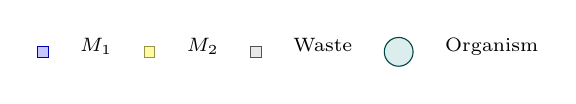
\begin{tikzpicture}
    \ChemostatSnapStyles
    \matrix[column sep=0.40cm, ampersand replacement=\&,
      nodes={inner sep=0pt, anchor=base}, row sep=0pt] {
        \node[csmballMone] {}; \&
        \node[font=\scriptsize] {$M_1$}; \&
        \node[csmballMtwo] {}; \&
        \node[font=\scriptsize] {$M_2$}; \&
        \node[csmballWaste] {}; \&
        \node[font=\scriptsize] {Waste}; \&
        \node[csorg] {}; \&
        \node[font=\scriptsize] {Organism}; \\
      };
  \end{tikzpicture}
  \\[4pt]
  \begin{tikzpicture}
    \ChemostatSnapStyles
    \matrix[column sep=0.40cm, ampersand replacement=\&,
      nodes={inner sep=0pt, anchor=base}, row sep=0pt] {
        \node[csorgMut] {}; \&
        \node[font=\scriptsize] {Mutant offspring}; \\
      };
  \end{tikzpicture}%
}

% Supp. Fig. S2 (diagram grid): chemostat symbols only.
\newcommand{\SimLoopVisLegend}{%
  \begin{center}
    \begin{tabular}{@{}c@{}}
      \SimLoopVisLegendGlyphs
    \end{tabular}
  \end{center}%
}

% Supp. Fig. S1 (combined flowchart): chemostat symbols only ($g$, $N_g$ on figure).
\newcommand{\SimLoopComboLegend}{\SimLoopVisLegend}

\newcommand{\SimLoopVisDiagram}[2][0.46\linewidth]{%
  \begin{center}
    \def\SimLoopVisVariant{#2}%
    \ifx\SimLoopVisVariant\Snap@energy
      \resizebox{\SimLoopVisEnergyWidthScale\dimexpr#1\relax}{!}{\ChemostatSnapEnergyPanel}%
    \else
      \resizebox{#1}{!}{\ChemostatSnapshot{}{#2}}%
    \fi
  \end{center}%
}

\newcommand{\SimLoopVisCell}[3][0.46\linewidth]{%
  \begin{center}
    {\scriptsize\bfseries #2\par\vspace{3pt}}
    \SimLoopVisDiagram[#1]{#3}%
  \end{center}%
}

\makeatother
